\documentclass[aspectratio=169, 9pt]{beamer}
\usetheme{metropolis}

\usepackage{xeCJK}
\setCJKmainfont{PingFang SC}
\setCJKsansfont{PingFang SC}
\setCJKmonofont{PingFang SC}

\usepackage{fontspec}
\setmonofont{Menlo}[Scale=0.82]
\usepackage{tikz}
\usetikzlibrary{arrows.meta, positioning, calc, shapes.geometric, shadows.blur}
\usepackage{graphicx}
\usepackage{booktabs}
\usepackage{array}
\usepackage{listings}
\usepackage{xcolor}

\graphicspath{{images/}}

% ── Color palette ──────────────────────────────────────────────────
\definecolor{primary}{HTML}{6C5CE7}
\definecolor{accent}{HTML}{00B894}
\definecolor{warning}{HTML}{E17055}
\definecolor{dark}{HTML}{2D3436}
\definecolor{light}{HTML}{DFE6E9}
\definecolor{muted}{HTML}{636E72}
\definecolor{codebg}{HTML}{F7F7FA}
\definecolor{erlred}{HTML}{D63031}
\definecolor{erlblue}{HTML}{0984E3}
\definecolor{nodegreen}{HTML}{00A884}

% ── Beamer theme ───────────────────────────────────────────────────
\setbeamercolor{normal text}{fg=dark,bg=white}
\setbeamercolor{frametitle}{fg=white,bg=primary}
\setbeamercolor{progress bar}{fg=accent,bg=light}
\setbeamercolor{alerted text}{fg=warning}
\setbeamercolor{block title}{fg=white,bg=primary}
\setbeamercolor{block body}{fg=dark,bg=primary!7}
\setbeamercolor{block title example}{fg=white,bg=accent}
\setbeamercolor{block body example}{fg=dark,bg=accent!7}
\setbeamertemplate{itemize item}{\color{accent}$\blacktriangleright$}
\setbeamertemplate{itemize subitem}{\color{primary}$\bullet$}
\setbeamertemplate{enumerate item}{\color{accent}\insertenumlabel.}
\metroset{progressbar=frametitle, numbering=fraction}

% ── Macros ─────────────────────────────────────────────────────────
\newcommand{\keypoint}[1]{\textbf{\color{primary}#1}}
\newcommand{\good}[1]{\textbf{\color{accent!80!black}#1}}
\newcommand{\warn}[1]{\textbf{\color{warning}#1}}
\newcommand{\bad}[1]{\textbf{\color{erlred}#1}}
\newcommand{\code}[1]{\texttt{#1}}
\newcommand{\imgslide}[3]{%
  \begin{frame}{#1}
    \begin{columns}[T,onlytextwidth]
      \column{0.58\textwidth}
      \centering
      \includegraphics[width=\linewidth,height=0.72\textheight,keepaspectratio]{#2}
      \column{0.38\textwidth}
      #3
    \end{columns}
  \end{frame}
}

\lstdefinelanguage{Erlang2}{
  keywords={module,export,application,supervisor,gen_server,gen_statem,case,of,end,fun,receive,after,true,false},
  sensitive=true,
  morecomment=[l]{\%},
  morestring=[b]",
  morestring=[b]'
}
\lstset{
  language=Erlang2,
  basicstyle=\ttfamily\scriptsize,
  keywordstyle=\color{primary}\bfseries,
  commentstyle=\color{muted}\itshape,
  stringstyle=\color{accent!70!black},
  backgroundcolor=\color{codebg},
  frame=single,
  framesep=1.5mm,
  rulecolor=\color{light},
  showstringspaces=false,
  breaklines=true,
  tabsize=2
}

\title{Erlang Observer UI}
\subtitle{从 Erlang Process 看见 BEAM，再进入 OTP 应用结构}
\author{}
\date{}

\begin{document}

% ── Title ──────────────────────────────────────────────────────────
\begin{frame}[plain]
  \begin{tikzpicture}[remember picture, overlay]
    \fill[primary!8] (current page.north west) rectangle (current page.south east);
    \fill[primary!15] (current page.north west) ++(1.7,-1.3) circle (2.7cm);
    \fill[accent!12]  (current page.south east) ++(-2.1,1.6) circle (3.0cm);
    \node[anchor=center, font=\fontsize{26}{32}\selectfont\bfseries, text=dark]
      at ([yshift=1.75cm]current page.center) {Erlang Observer UI};
    \node[anchor=center, font=\Large, text=primary!80]
      at ([yshift=0.55cm]current page.center) {先看见 Erlang Process，再理解 OTP 如何组织它们};
    \node[anchor=center, font=\large\bfseries, text=accent!80!black]
      at ([yshift=-0.35cm]current page.center) {Erlang 最大的特色，是可以被运行时直接观察的轻量级 Process};
    \draw[accent, line width=1.5pt]
      ([yshift=-1.15cm, xshift=-4.8cm]current page.center)
      -- ([yshift=-1.15cm, xshift=4.8cm]current page.center);
    \node[anchor=south, font=\scriptsize, text=dark!45]
      at ([yshift=0.4cm]current page.south)
      {理解路径：Process \enspace|\enspace Observer \enspace|\enspace 为什么需要 OTP \enspace|\enspace Applications};
  \end{tikzpicture}
\end{frame}

% ── Process first ──────────────────────────────────────────────────
\begin{frame}{进入 OTP 之前，先看 Erlang Process}
  \begin{columns}[T,onlytextwidth]
    \column{0.52\textwidth}
    \begin{alertblock}{先从可视化的运行时对象开始}
      要理解 Observer 如何可视化 OTP，先认识 Erlang 最核心的抽象：\keypoint{Erlang Process}。
    \end{alertblock}
    \begin{block}{为什么它重要？}
      \begin{itemize}
        \item Erlang 能支撑大量连接，核心不是靠大量 OS thread
        \item Erlang 是面向进程编程：连接、会话、任务、状态都可以建模成 process
        \item BEAM VM 内部运行的是大量 Erlang process
        \item 它们是 Erlang 并发模型的基本单位
      \end{itemize}
    \end{block}
    \column{0.42\textwidth}
    \begin{exampleblock}{先建立直觉}
      \centering
      \Large
      先看 Process 是什么\par
      再看怎么观察它\par
      最后再问：\par
      \good{这么多 Process 怎么管理？}
    \end{exampleblock}
  \end{columns}
\end{frame}

\begin{frame}{一个 Erlang VM 里可以有很多 Process}
  \centering
  \begin{tikzpicture}[
    box/.style={draw, rounded corners=2mm, thick, fill=primary!7, minimum width=3.2cm, minimum height=0.75cm},
    proc/.style={draw, rounded corners=1.5mm, thick, fill=accent!10, minimum width=1.9cm, minimum height=0.55cm, font=\small},
    label/.style={font=\bfseries\large, text=dark}
  ]
    \node[label] at (-3.8,2.2) {Linux};
    \node[box] (chrome) at (-3.8,1.1) {Chrome};
    \node[box] (redis) at (-3.8,0.0) {Redis};
    \node[box] (nginx) at (-3.8,-1.1) {Nginx};
    \node[font=\small, text=muted] at (-3.8,-2.0) {OS Process};

    \draw[very thick, primary!50] (0,-2.4) -- (0,2.6);

    \node[label] at (3.6,2.2) {Erlang VM};
    \foreach \x/\y in {2.3/1.2,3.6/1.2,4.9/1.2,2.3/0.25,3.6/0.25,4.9/0.25,2.3/-0.7,3.6/-0.7,4.9/-0.7,2.95/-1.65,4.25/-1.65} {
      \node[proc] at (\x,\y) {Process};
    }
    \node[font=\small, text=muted, align=center] at (3.6,-2.35) {几十万甚至上百万个\par Erlang Process};
  \end{tikzpicture}

  \vspace{0.25cm}
  \good{因为 Erlang 鼓励用 Process 建模系统，一个 VM 内部自然可能出现大量 Erlang Process。}
\end{frame}

\begin{frame}{它叫 Process，但不是操作系统进程}
  \begin{columns}[T,onlytextwidth]
    \column{0.48\textwidth}
    \begin{block}{OS Process / OS Thread}
      \begin{itemize}
        \item 操作系统管理
        \item 相对重量级
        \item 上下文切换成本更高
        \item 资源隔离边界更强
      \end{itemize}
    \end{block}
    \column{0.48\textwidth}
    \begin{exampleblock}{Erlang Process}
      \begin{itemize}
        \item 语言级并发实体
        \item 由 BEAM VM 调度
        \item 非常轻量
        \item 适合海量并发建模
      \end{itemize}
    \end{exampleblock}
  \end{columns}
  \vspace{0.25cm}
  \centering
  \warn{可以近似理解为 Go goroutine 或协程，但更准确地说：它是 BEAM 管理的 lightweight process。}
\end{frame}

\begin{frame}{为什么说 Erlang Process 很神奇？}
  \begin{columns}[T,onlytextwidth]
    \column{0.44\textwidth}
    \centering
    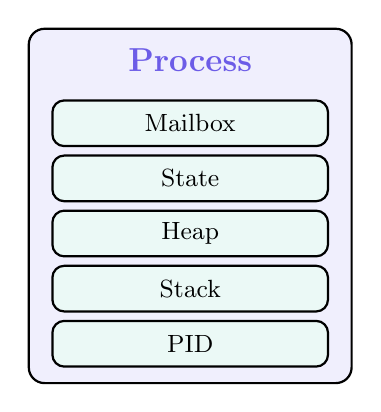
\begin{tikzpicture}[
      part/.style={draw, rounded corners=1.5mm, thick, fill=accent!8, minimum width=3.5cm, minimum height=0.58cm, font=\small}
    ]
      \node[draw, rounded corners=2mm, thick, fill=primary!10, minimum width=4.1cm, minimum height=4.5cm] (p) at (0,0) {};
      \node[font=\bfseries\large, text=primary] at (0,1.85) {Process};
      \node[part] at (0,1.05) {Mailbox};
      \node[part] at (0,0.35) {State};
      \node[part] at (0,-0.35) {Heap};
      \node[part] at (0,-1.05) {Stack};
      \node[part] at (0,-1.75) {PID};
    \end{tikzpicture}
    \column{0.52\textwidth}
    \begin{block}{每个 Process 都有自己的运行现场}
      \begin{itemize}
        \item 自己的邮箱：接收消息
        \item 自己的状态：保存业务上下文
        \item 自己的堆和栈：独立执行
        \item 自己的 PID：可以被定位和通信
      \end{itemize}
    \end{block}
    \begin{alertblock}{通信方式}
      Process 之间不共享内存，主要通过消息传递协作。
    \end{alertblock}
  \end{columns}
\end{frame}

\begin{frame}{最神奇的地方：不仅有 Process，而且还能直接看到它}
  \begin{columns}[T,onlytextwidth]
    \column{0.50\textwidth}
    \begin{block}{Observer 能看到运行现场}
      \begin{itemize}
        \item Processes 列表
        \item PID / registered name
        \item Mailbox / MsgQ
        \item Memory / reductions
        \item Stack Trace / Current Function
      \end{itemize}
    \end{block}
    \column{0.46\textwidth}
    \begin{exampleblock}{这句话很关键}
      \centering
      \Large
      很多语言都有“轻量并发”。\par\vspace{0.2cm}
      但很少有语言，\par
      把并发单元的运行现场\par
      \good{原生展示出来}。
    \end{exampleblock}
  \end{columns}
\end{frame}

\imgslide{Processes：先看见 Erlang process}{Applications_process_list.png}{%
  \begin{block}{进程为什么重要？}
    \begin{itemize}
      \item Erlang process 是 BEAM 里的并发建模单位
      \item worker 最终都会落到具体 BEAM process
      \item 可观察 memory / reductions / MsgQ
      \item 可以双击进入 Process Information
    \end{itemize}
  \end{block}
  \begin{exampleblock}{这不是 Debugger}
    这是运行中的现场：每个 process 的 PID、内存、消息队列和当前执行信息都可以被直接观察。
  \end{exampleblock}
}

\imgslide{Process Internals：Messages / Dictionary / Stack Trace}{Process_Messages.png}{%
  \begin{block}{进程内部三件事}
    \begin{itemize}
      \item Messages：mailbox 中未处理消息
      \item Dictionary：进程字典
      \item Stack Trace：当前调用栈
    \end{itemize}
  \end{block}
  \begin{exampleblock}{排查意义}
    消息堆积、进程卡住、状态异常，都能从 process 级别继续向内看。
  \end{exampleblock}
}

\imgslide{Process Data：通过 Table Viewer 看 ETS / DETS}{Table_Viewer.png}{%
  \begin{block}{表数据观察}
    \begin{itemize}
      \item ETS table
      \item DETS table
      \item cache / storage 模块常用
    \end{itemize}
  \end{block}
  \begin{alertblock}{和进程主线的关系}
    \code{data\_cache}、\code{data\_store} 这类 worker process 背后的表数据，也属于进程观察继续深入的一部分。
  \end{alertblock}
}

% ── Start ──────────────────────────────────────────────────────────
\begin{frame}{如果有几十万个 Process，怎么办？}
  \begin{columns}[T,onlytextwidth]
    \column{0.50\textwidth}
    \begin{alertblock}{为什么会有这么多 Process？}
      Erlang 是面向进程编程：一个连接、一个会话、一个 worker、一个状态持有者，都可以是独立 process。
    \end{alertblock}
    \begin{alertblock}{自然产生的问题}
      每个 Process 都要自己管理？谁负责启动？谁负责重启？谁负责组织依赖关系？
    \end{alertblock}
    \begin{block}{答案不是手写一堆管理代码}
      \begin{itemize}
        \item \code{application} 负责组织系统
        \item \code{supervisor} 负责管理进程生命周期
        \item \code{worker} 真正执行业务
      \end{itemize}
    \end{block}
    \column{0.46\textwidth}
    \begin{exampleblock}{这时再引出 OTP}
      \centering
      \Large
      Process 是并发基本单位。\par
      OTP 解决的是：\par
      \good{大量 Process 如何组织和容错}。
    \end{exampleblock}
  \end{columns}
\end{frame}

\begin{frame}{Let it crash：不是放任崩溃，而是有人接住}
  \begin{columns}[T,onlytextwidth]
    \column{0.50\textwidth}
    \begin{block}{Application 的角色}
      \begin{itemize}
        \item 把一组进程组织成一个可启动的系统
        \item 定义顶层 supervisor 入口
        \item 让系统有清晰的运行边界
      \end{itemize}
    \end{block}
    \begin{block}{Supervisor 的角色}
      \begin{itemize}
        \item 监控 worker process 是否退出
        \item 按策略决定重启谁
        \item 把局部失败限制在可恢复范围内
      \end{itemize}
    \end{block}
    \column{0.46\textwidth}
    \begin{exampleblock}{核心哲学}
      \centering
      \Large
      Process 负责隔离失败。\par\vspace{0.2cm}
      Supervisor 负责恢复失败。\par\vspace{0.2cm}
      Application 负责组织系统。\par\vspace{0.35cm}
      \good{这才是 let it crash 的工程含义。}
    \end{exampleblock}
  \end{columns}
  \vspace{0.2cm}
  \centering
  \warn{后面讲 OTP 时，会展开 supervisor 如何发现退出、选择重启策略、控制重启强度。}
\end{frame}

\begin{frame}[fragile]{启动 demo：用 Observer 观察一个 OTP 应用}
  \begin{columns}[T,onlytextwidth]
    \column{0.50\textwidth}
    \begin{block}{启动 demo 节点}
\begin{lstlisting}
cd bilibili_erlang/observer/full_otp_app
rebar3 shell --sname application_demo
\end{lstlisting}
    \end{block}
    \begin{block}{启动应用和 Observer}
\begin{lstlisting}
application:ensure_all_started(full_otp_app).
observer:start().
\end{lstlisting}
    \end{block}
    \column{0.46\textwidth}
    \centering
    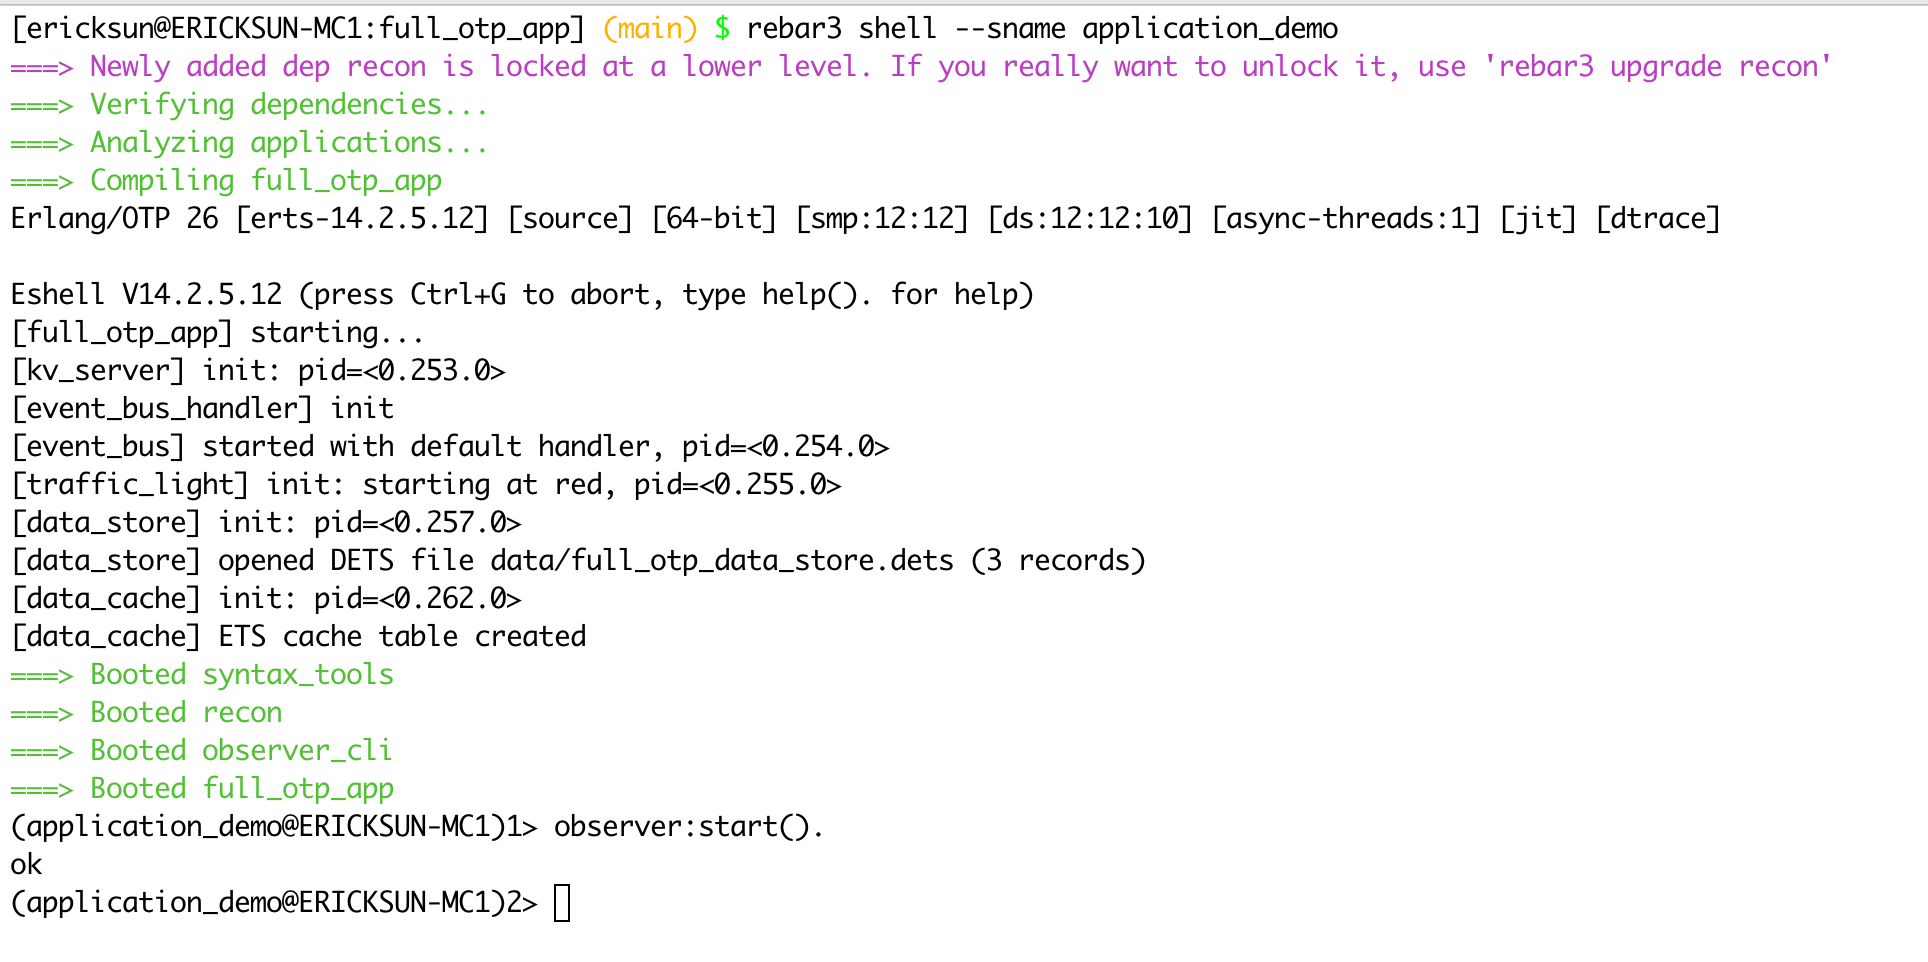
\includegraphics[width=\linewidth,height=0.63\textheight,keepaspectratio]{observer_start.png}
  \end{columns}
\end{frame}

% ── Applications as focus ──────────────────────────────────────────
\begin{frame}{正式进入 OTP：从 Applications 看 Process 如何被组织}
  \begin{columns}[T,onlytextwidth]
    \column{0.48\textwidth}
    \begin{block}{为什么现在看 Applications？}
      \begin{itemize}
        \item 刚才的问题是：大量 process 怎么管理？
        \item 更进一步：process 崩溃后谁来恢复？
        \item OTP 从 application 组织系统
        \item application 下面是 supervisor tree
        \item supervisor 管理 worker process 的生命周期
        \item gen\_server / gen\_statem 最终都落到 process
      \end{itemize}
    \end{block}
    \column{0.48\textwidth}
    \begin{exampleblock}{Applications 页面给出主线}
      \centering
      \code{application}\par
      $\downarrow$\par
      \code{supervisor tree}\par
      $\downarrow$\par
      \code{worker process}\par
      $\downarrow$\par
      \code{mailbox + state + tables}
    \end{exampleblock}
  \end{columns}
\end{frame}

\begin{frame}{full\_otp\_app：一个完整 OTP 小工程}
  \begin{columns}[T,onlytextwidth]
    \column{0.52\textwidth}
    \begin{block}{为什么用这个 demo？}
      \begin{itemize}
        \item \code{full\_otp\_app} 是一个 application
        \item 入口进程是 root supervisor
        \item supervisor 下面既有 worker，也有 child supervisor
        \item 方便在 Observer 里看到真实 supervisor tree
      \end{itemize}
    \end{block}

    \column{0.44\textwidth}
    \begin{exampleblock}{覆盖的 OTP 组件}
      \begin{itemize}
        \item \code{application}
        \item \code{supervisor} / 子 \code{supervisor}
        \item \code{gen\_server}
        \item \code{gen\_statem}
      \end{itemize}
    \end{exampleblock}
  \end{columns}

  \vspace{0.15cm}
  \good{这不是为了业务复杂度，而是为了把常见 OTP 运行时结构一次性展示出来。}
\end{frame}

\begin{frame}{OTP 层级：从 Application 组织到 BEAM Process}
  \centering
  % application-hierarchy-body.tex — full_otp_app application hierarchy diagram
% Shared TikZ source used by observer_ui_beamer.tex and standalone preview.

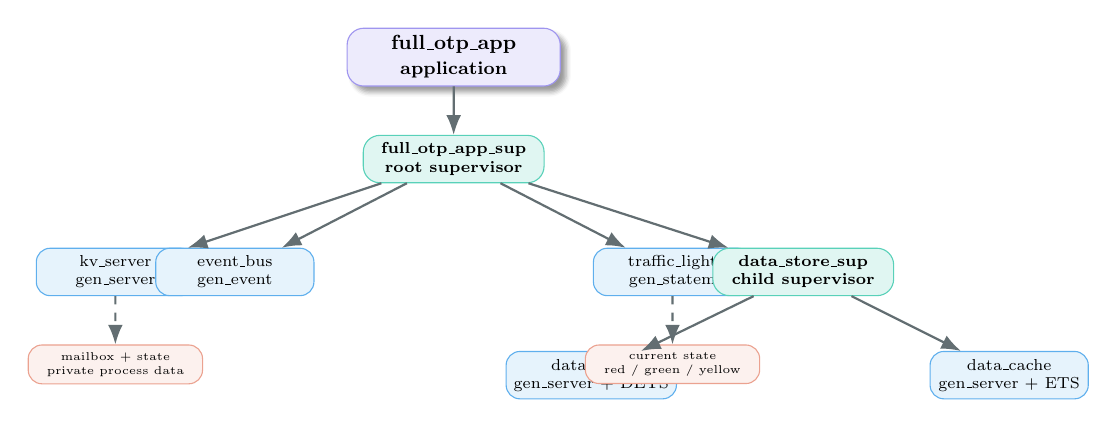
\begin{tikzpicture}[
  scale=0.82, transform shape,
  node distance=0.75cm and 1.05cm,
  app/.style={rounded corners=6pt, draw=primary!65, fill=primary!12, minimum width=3.3cm, minimum height=0.75cm, align=center, font=\small\bfseries, blur shadow},
  sup/.style={rounded corners=6pt, draw=accent!65, fill=accent!12, minimum width=2.8cm, minimum height=0.7cm, align=center, font=\scriptsize\bfseries},
  worker/.style={rounded corners=5pt, draw=erlblue!65, fill=erlblue!10, minimum width=2.45cm, minimum height=0.62cm, align=center, font=\scriptsize},
  detail/.style={rounded corners=5pt, draw=warning!65, fill=warning!10, minimum width=2.7cm, minimum height=0.56cm, align=center, font=\tiny},
  arrow/.style={-{Latex[length=2.5mm]}, thick, color=muted}
]
  \node[app] (app) {full\_otp\_app\\\footnotesize application};

  \node[sup, below=of app] (root) {full\_otp\_app\_sup\\root supervisor};

  \node[worker, below left=1.0cm and 2.6cm of root] (kv) {kv\_server\\gen\_server};
  \node[worker, below left=1.0cm and 0.75cm of root] (event) {event\_bus\\gen\_event};
  \node[worker, below right=1.0cm and 0.75cm of root] (traffic) {traffic\_light\\gen\_statem};
  \node[sup, below right=1.0cm and 2.6cm of root] (dataSup) {data\_store\_sup\\child supervisor};

  \node[worker, below left=0.85cm and 0.55cm of dataSup] (store) {data\_store\\gen\_server + DETS};
  \node[worker, below right=0.85cm and 0.55cm of dataSup] (cache) {data\_cache\\gen\_server + ETS};

  \node[detail, below=0.75cm of kv] (kvState) {mailbox + state\\private process data};
  \node[detail, below=0.75cm of traffic] (fsmState) {current state\\red / green / yellow};

  \draw[arrow] (app) -- (root);
  \draw[arrow] (root) -- (kv);
  \draw[arrow] (root) -- (event);
  \draw[arrow] (root) -- (traffic);
  \draw[arrow] (root) -- (dataSup);
  \draw[arrow] (dataSup) -- (store);
  \draw[arrow] (dataSup) -- (cache);
  \draw[arrow, dashed] (kv) -- (kvState);
  \draw[arrow, dashed] (traffic) -- (fsmState);
\end{tikzpicture}


  \vspace{0.2cm}
  \good{OTP 的意义，是把大量 Process 组织成可以启动、监督、重启的系统结构。}
\end{frame}

\imgslide{Applications：看 OTP 如何组织运行中的 Process}{Applications.png}{%
  \begin{block}{左侧 application 列表}
    \begin{itemize}
      \item 系统 application：\code{kernel}、\code{stdlib}、\code{ssl}
      \item 业务 application：\code{full\_otp\_app}
      \item 每个 application 都是 OTP 系统组织单位
    \end{itemize}
  \end{block}
  \begin{exampleblock}{本页要强调}
    Applications 页面不是起点，而是答案：它告诉我们大量 Process 在 OTP 里如何被组织成一个系统。
  \end{exampleblock}
}

\imgslide{full\_otp\_app：把代码映射到运行时}{Applications_app.png}{%
  \begin{block}{选中 demo application 后}
    \begin{itemize}
      \item 看 application 状态
      \item 看启动信息和依赖
      \item 进入 supervision tree
      \item 连接到 \code{.app.src} 配置
    \end{itemize}
  \end{block}
  \begin{alertblock}{这一页的意义}
    \code{full\_otp\_app} 不是一个静态配置名，而是运行中的 OTP application，可以继续展开到 supervisor 和 worker process。
  \end{alertblock}
}

\imgslide{Supervisor Tree：Applications 页面最重要的能力}{Applications_app_supervisor.png}{%
  \begin{block}{为什么这张图最关键？}
    \begin{itemize}
      \item application 下面是 root supervisor
      \item supervisor 管理 worker process
      \item worker 对应 gen\_server / gen\_statem
      \item OTP 的容错结构直接可视化
    \end{itemize}
  \end{block}
  \begin{exampleblock}{一句话结论}
    supervisor tree 不是概念图，而是正在运行的进程关系图。
  \end{exampleblock}
}

\imgslide{Nested Supervisor：OTP 可以分层组织系统}{Applications_app_supervisor_second.png}{%
  \begin{block}{data\_store\_sup}
    \begin{itemize}
      \item 子 supervisor 继续管理子系统
      \item \code{data\_store} 负责 DETS
      \item \code{data\_cache} 负责 ETS cache
      \item 对应 \code{rest\_for\_one} 策略
    \end{itemize}
  \end{block}
  \begin{alertblock}{应用层级的意义}
    大系统不是一堆散乱进程，而是 application + supervisor tree 组织起来。
  \end{alertblock}
}

% ── Worker process deep dive ───────────────────────────────────────
\begin{frame}{从 OTP worker 回到具体 Process}
  \begin{columns}[T,onlytextwidth]
    \column{0.48\textwidth}
    \begin{block}{进程内部}
      \begin{itemize}
        \item Process Information：PID / links / monitors
        \item State：callback 返回后的私有状态
        \item Messages：mailbox 里的未处理消息
        \item Dictionary / Stack Trace：排查进程现场
      \end{itemize}
    \end{block}
    \column{0.48\textwidth}
    \begin{exampleblock}{进程关联资源}
      \begin{itemize}
        \item worker 可能拥有 ETS table
        \item worker 可能打开 DETS table
        \item Table Viewer 是从进程继续看数据面的补充
      \end{itemize}
    \end{exampleblock}
  \end{columns}
  \vspace{0.2cm}
  \centering
  \good{前面先认识了 Process；现在从 Applications 追到 worker，是把 OTP 结构重新落回具体 Process。}
\end{frame}

\imgslide{gen\_server：查看 kv\_server 进程}{Applications_app_gen_server_process.png}{%
  \begin{block}{Process Information}
    \begin{itemize}
      \item PID / registered name
      \item links / monitors
      \item message queue
      \item reductions / memory
    \end{itemize}
  \end{block}
  \begin{alertblock}{教学重点}
    \code{gen\_server} 不是对象，它是有 mailbox 和私有状态的进程。
  \end{alertblock}
}

\imgslide{State：看见 gen\_server 的私有状态}{Applications_app_gen_server_state.png}{%
  \begin{block}{State tab}
    \begin{itemize}
      \item 展示当前 process state
      \item callback 返回的新 state 会反映到这里
      \item 适合演示 \code{kv\_server:put/2}
    \end{itemize}
  \end{block}
  \begin{exampleblock}{Observer 的教学价值}
    学生可以把 callback 返回值和运行时状态直接对应起来。
  \end{exampleblock}
}

\imgslide{gen\_statem：状态机也能直接观察}{Applications_app_traffic_light_state.png}{%
  \begin{block}{traffic\_light}
    \begin{itemize}
      \item 当前状态：red / green / yellow
      \item 状态数据：map
      \item timeout / event 触发状态迁移
    \end{itemize}
  \end{block}
  \begin{alertblock}{适合课堂演示}
    执行 \code{traffic\_light:next().} 后刷新 State，状态变化一目了然。
  \end{alertblock}
}

\begin{frame}{小结：这条理解路径是什么？}
  \begin{block}{从 Process 到 OTP，再回到 Observer}
    \begin{itemize}
      \item Erlang Process 是 BEAM 的轻量级并发实体，不是 OS process
      \item Observer 能直接看到 process 的运行现场
      \item 大量 process 需要被组织和管理，于是引出 OTP
      \item application / supervisor / worker 把 process 组织成系统
      \item Applications 页面把这个 OTP 结构变成运行时可见对象
    \end{itemize}
  \end{block}
  \begin{exampleblock}{最重要的一句话}
    \centering
    \Large
    Observer 把 Erlang Process 和 OTP 结构，变成了\good{运行时可见的系统}。
  \end{exampleblock}
\end{frame}

\end{document}
